\documentclass[a4paper,12pt]{article}

\usepackage{graphicx}
\usepackage[utf8]{inputenc}
\usepackage[T1]{fontenc}
\usepackage{amsmath}
\usepackage{caption}
\usepackage{subcaption}

\title{ Mecânica Clássica I  Coordenadas - Esféricas}
\author{Anderson Thiago \\ André Del Bianco Giuffrida \\  Gabriela Curti \\ Priscila França Guidini 
}
\date{}
\begin{document}
	\maketitle
	\paragraph \indent Para tratar problemas de Mecânica Clássica, é comum ultilizar-mos três sistemas de coordenadas: Esféricas, Cilindricas e Cartesianas.\\
	\indent A maior diferença entre coordenadas esféricas e cartesianas é visualizar que os versores $\hat{r}, \hat{\theta}, \hat{\varphi}$ variam com o tempo, diferente de $\hat{i},\hat{j},\hat{k}$ que são fixos, de modo que:
	\begin{figure}[h]
		\begin{center}
			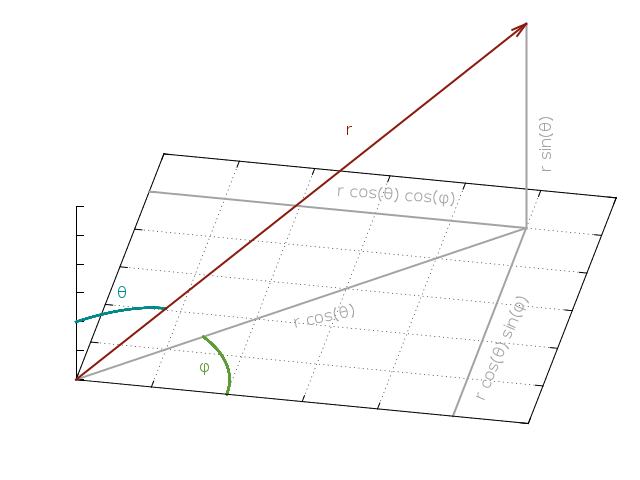
\includegraphics[scale=0.3]{SphericalCoordinates.png} 
		\end{center}
	\end{figure} 
	\begin{equation*}
		\begin{cases}
			x = r sin(\theta) cos(\varphi)  &\\
			y = r sin(\theta) sin(\varphi) &\\
			z = r cos(\theta) &
		\end{cases}
	\end{equation*}
	
	
	  
	
	 Pela Figura podemos ver que a posição é dada pelo vetor $\vec{r}$, onde:
	 
	 \[ \vec{r} = r\hat{r} \] \\
	 e:
	 	\[ \vec{r} = r sin(\theta) cos(\varphi) \hat{i} + r sin(\theta) sin(\varphi) \hat{j} + r cos(\theta) \hat{k} \]
	 	de modo que $\hat{r}$ :
	 	\[ \hat{r} = sin(\theta) cos(\varphi) \hat{i} + sin(\theta) sin(\varphi) \hat{j} + cos(\theta) \hat{k} \] 
	 	
além disso temos:	 	
	 	\[ \hat{\varphi} = \hat{k}\quad \text{x}\quad \hat{r}  = -sin(\varphi) \hat{i} + cos(\varphi) \hat{j}\]
	 	e
	 	\[ \hat{\theta} = \hat{\varphi}\quad  \text{x} \quad   \hat{r} = 
	 	cos(\theta) cos(\varphi) \hat{i} + cos(\theta) sin(\varphi) \hat{j} -  sin(\theta) \hat{k}\]
	 \paragraph \indent	Com os versores definidos podemos calcular a aceleração e a velocidade em coordenadas esféricas.
	 	
	 	\[ \vec{v} = \frac{d \vec{r} }{dt} = \dot{\vec{r}} = \dot{r} \hat{r} + r\dot{\theta} \hat{\theta}+ ( r \dot{\varphi} sin(\theta) ) \hat{\varphi} \]
	 	
	\begin{eqnarray*}
	\vec{a} = \frac{ d^2 \vec{r} }{ dt^2 } = &+&( \ddot{\vec{r}}  - r \dot{\theta}^2 -r\dot{\varphi}^2 sin(\theta)^2 )\hat{r} \\ 
	&+&( r \ddot{\theta} + 2 \dot{r} \dot{\theta} -r\dot{\varphi}^2 sin(\theta) cos(\theta) )\hat{\theta} \\
	 &+& ( r \ddot{\varphi} sin(\theta) + 2\dot{r} \dot{\varphi} sin(\theta) + 2r\dot{\theta} \dot{\varphi} cos(\theta) ) \hat{\varphi} 
	\end{eqnarray*}
	
	 	
	 Vemos nas equações acima que alguns termos são reconheciveis como: \\

 $\dot{r}\hat{r}$  \indent  Velocidade radial: velocidade com que o objeto se aproxima ou se afasta da origem na direção radial. \\
	
 $ r \dot{\theta}\hat{\theta} \quad\text{e}\quad rsin(\theta)\dot{\varphi}\hat{\varphi}$ \indent Velocidade tangencial: é perpendicular a $\hat{r}$ sendo orientada na direção azimutal ou polar. \\

$\ddot{r} \dot{\theta}^2 r \hat{r} $ \indent Aceleração centripeta: Característico de movimentos curvilíneos ou circulares. Ela é perpendicular à velocidade e aponta para o centro da trajetória. \\

$ r \ddot{\theta} \hat{\theta} $\indent Aceleração angular: é a variação da velocidade angular no tempo \\

$ 2\dot{r} \dot{\theta} \hat{\theta} \quad \text{e} \quad 2\dot{r}sin(\theta)\dot{\varphi}\hat{\varphi} $ \indent Aceleração de Coriolis: Aceleração de um corpo que se move em relação a um sistema de referência, medida em outro sistema de referência que apresenta uma aceleração angular em relação ao primeiro. \\


\end{document}
